\section{Results}\label{results}

In this section, we present our results on how VSFs reflect the distribution of turbulent power within molecular clouds.

\subsection{Examples}\label{results:example}

Fig.~\ref{pic:results:vsf_example} shows three examples of VSFs, (a) cloud \texttt{M4} at $t$~=~1.2~Myr after self-gravity has been activated in the simulations, (b) \texttt{M3} at $t$~=~3.5~Myr, and (c) \texttt{M3} at $t$~=~4.0~Myr.
All plots show the \textbf{density-weighted} VSFs of orders $p$~=~1--3.
The solid lines show the fitted power-law relations as given in Eq.~(\ref{equ:method:fitting}).

\begin{figure*}[!htb]
	\centering
	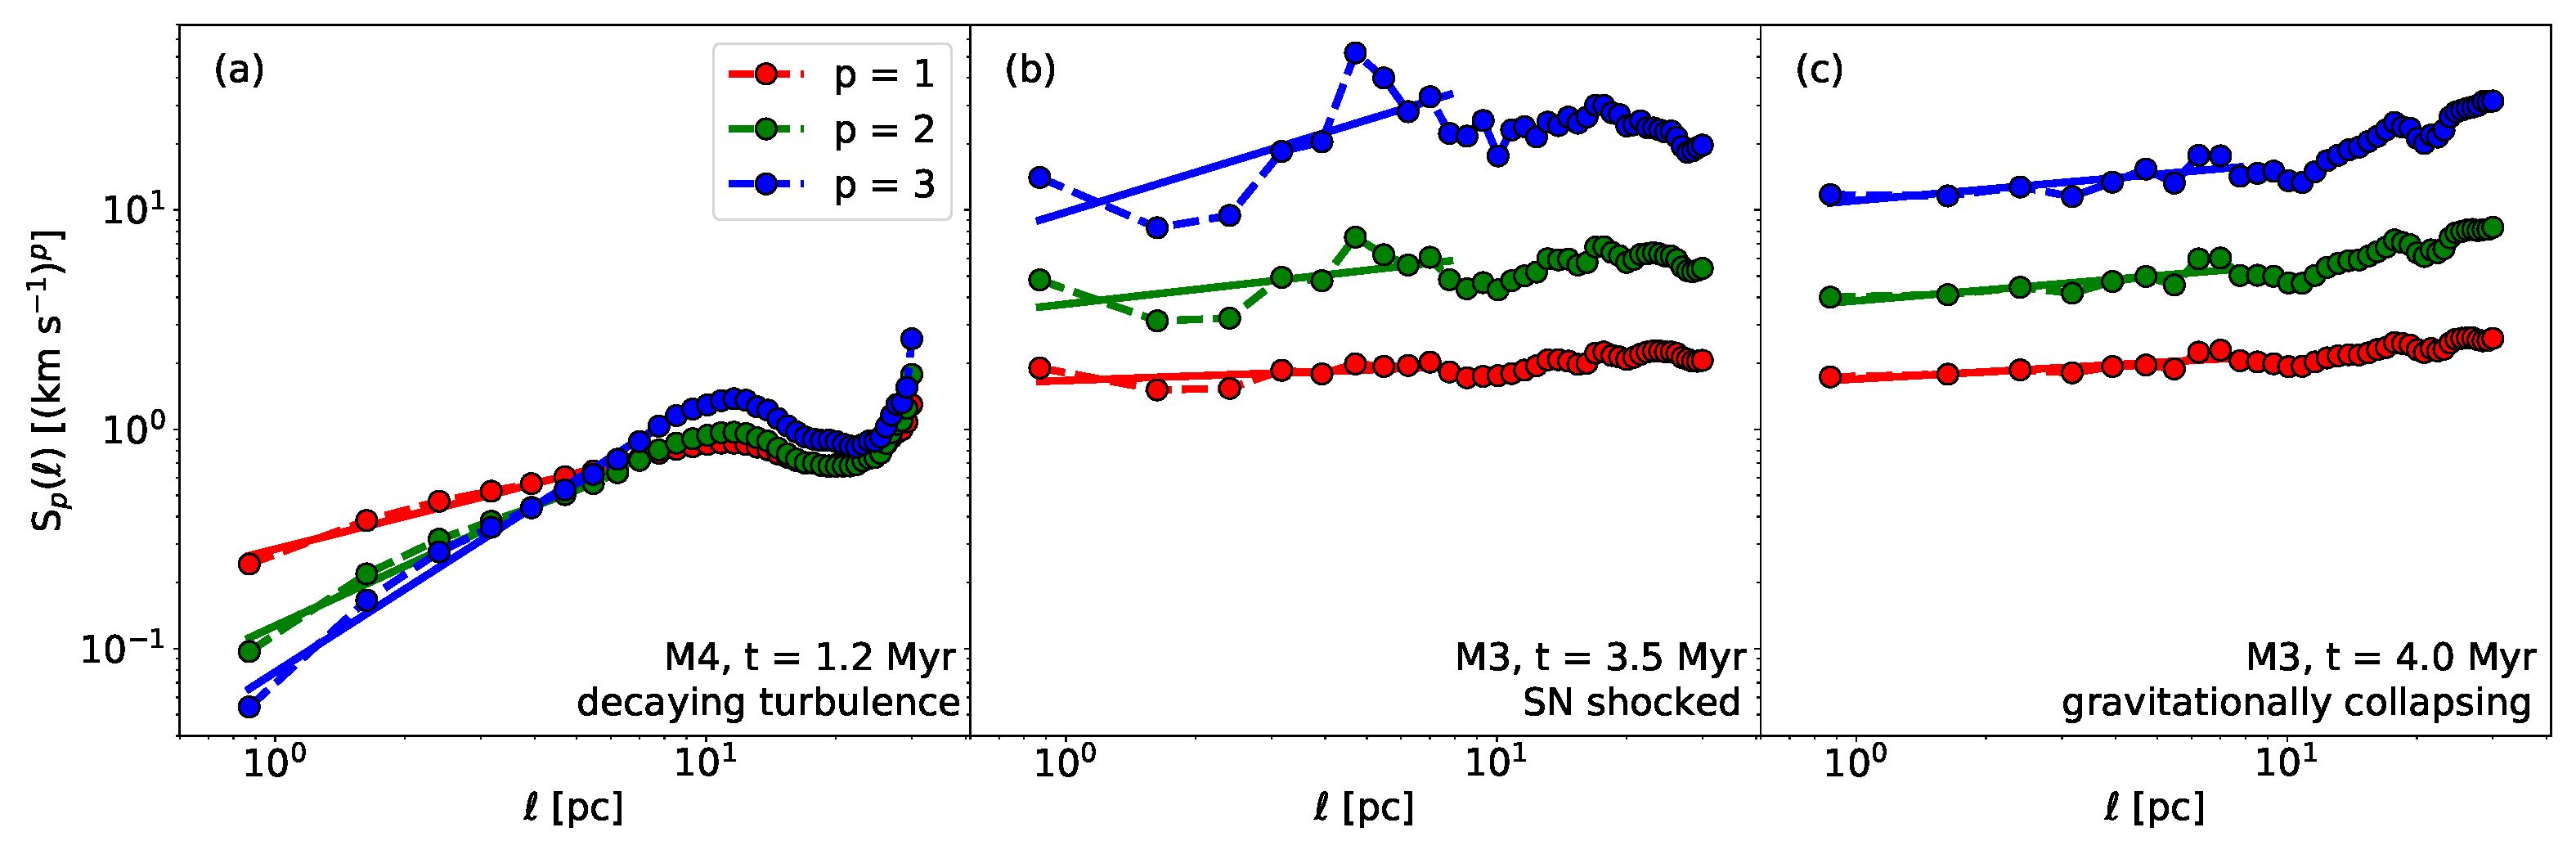
\includegraphics[width=\textwidth]{vsf_example.pdf}
	\caption{Examples of velocity structure functions as function of the lag scale $\ell$ and order $p$. 
		The dots (connected by dashed lines) show the values computed from the simulation.
		The solid lines represent the power-law relations fitted to the respective structure functions.
	}
	\label{pic:results:vsf_example}
\end{figure*}

The examples demonstrate that, in general, the measured VSFs cannot be described by a single power-law relation over the entire range of $\ell$.
Instead they are composed of roughly three different regimes: 
one at small scales at $\ell \lesssim$~3~pc, a second one within 3~pc~$\lesssim \ell \lesssim$~10--15~pc, and the last one at large scales with $\ell >$~15~pc.
\textbf{We find that} only the small and intermediate ranges may be represented by a common power-law relation.
On larger scales, one observes a local minimum before the VSFs either increase or stagnate.
Thus, in this context the VSF is an accurate tool to measure the size of a molecular cloud.
On smaller scales, which correspond to individual clumps and cores, one sees significant differences.

The examples in Fig.~\ref{pic:results:vsf_example} illustrate how VSFs react to different scenarios that affect the turbulent structure of the entire clouds. 
\textbf{Fig.~\ref{pic:results:vsf_example}(a) shows the case where turbulence is driven on large scales and naturally decays towards smaller scales.
This is the most common behavior seen in all three MCs within the first $\sim$1.5~Myr of the simulations.}
During this interval of time the clouds experience the effect of self-gravity for the first time in their evolution and need to adjust to this new condition.
Until this is the case, their VSFs are dominated by the freely cascading turbulence that previously dominated the kinetic structure of the clouds.
Furthermore, this implies that we can only reliably examine turbulence within the simulations after 1.5~Myr and carefully need to take this into account in the further discussion \citep[see][]{IbanezMejia2017,Seifried2017b}.

The other examples represent the clouds at later stages of their evolution when the VSFs are dominated by sources that drive the \textbf{flow} within the clouds in a more extreme way.
Fig.~\ref{pic:results:vsf_example}(b) shows the VSF of \texttt{M3} at a time when the cloud has just been hit by a SN shock front. 
One clearly sees how the amplitude of the VSFs is increased by one to two orders of magnitudes compared to the previous example.
Especially the power \textbf{at small scales ($\ell \lesssim$ few parsecs) is highly amplified as a result of the shock.} 
Despite the increase of turbulent power at small scales, a large amount of energy is injected at large scales, as well.
All this results in a \textbf{steeper slope of the VSF.}
However, the effect of SN shocks last for only a short period of time (see below).

The last example, Fig.~\ref{pic:results:vsf_example}(c), demonstrates the imprint of gravitational contraction.
Here, the VSF is almost flat, or even slightly increasing towards smaller separation scales. 
This kind of profile is typical for gas that is self-gravitationally contracting \citep{Boneberg2015,Burkhart2015} since gas moves into the inner regions of the cloud, reducing the average lag distances, but not necessarily the relative velocities.
The latter may even be accelerated by the infall.
As a consequence, large amounts of kinetic energy are transferred to smaller scales which flattens the corresponding VSF.

\subsection{Time Evolution}\label{results:normal}

Fig.~\ref{pic:results:zeta_all}(a) plots the time evolution of the power-law index $\zeta(p)$ fit to the \textbf{density-weighted} VSF obtained for each cloud, and each order $p$.
The figure shows several interesting features.
First, initially, at $t$~=~0~Myr, all calculated values of $\zeta$ are above the predicted values (see Eqs.~(\ref{equ:method:she}) and~(\ref{equ:method:boldyrev})).
\textbf{This suggests that we are seeing excess power at large scales from the initial convergent flows that formed the clouds.}
Second, $\zeta$ for all orders decreases with time as the clouds gravitationally collapse.
\textbf{Distributed gravitational collapse causes an increase in relative velocities at increasingly small scales as material falls into filaments and nodes.  The increase in small-scale power leads to a flattening of the VSF and thus a decrease in $\zeta$.}
Third, occasionally one observes bumps and dips in all orders of VSFs (e.g., \texttt{M3} or \texttt{M8} around $t$~=~1.7~Myr). 
These features only last for short periods of time (up to 0.6~Myr), but set in \textbf{rather abruptly and represent sudden changes in large-scale power that change the VSF slope. }

\begin{figure*}[!htb]
	\centering  
  
  \begin{subfigure}[c]{\textwidth}
      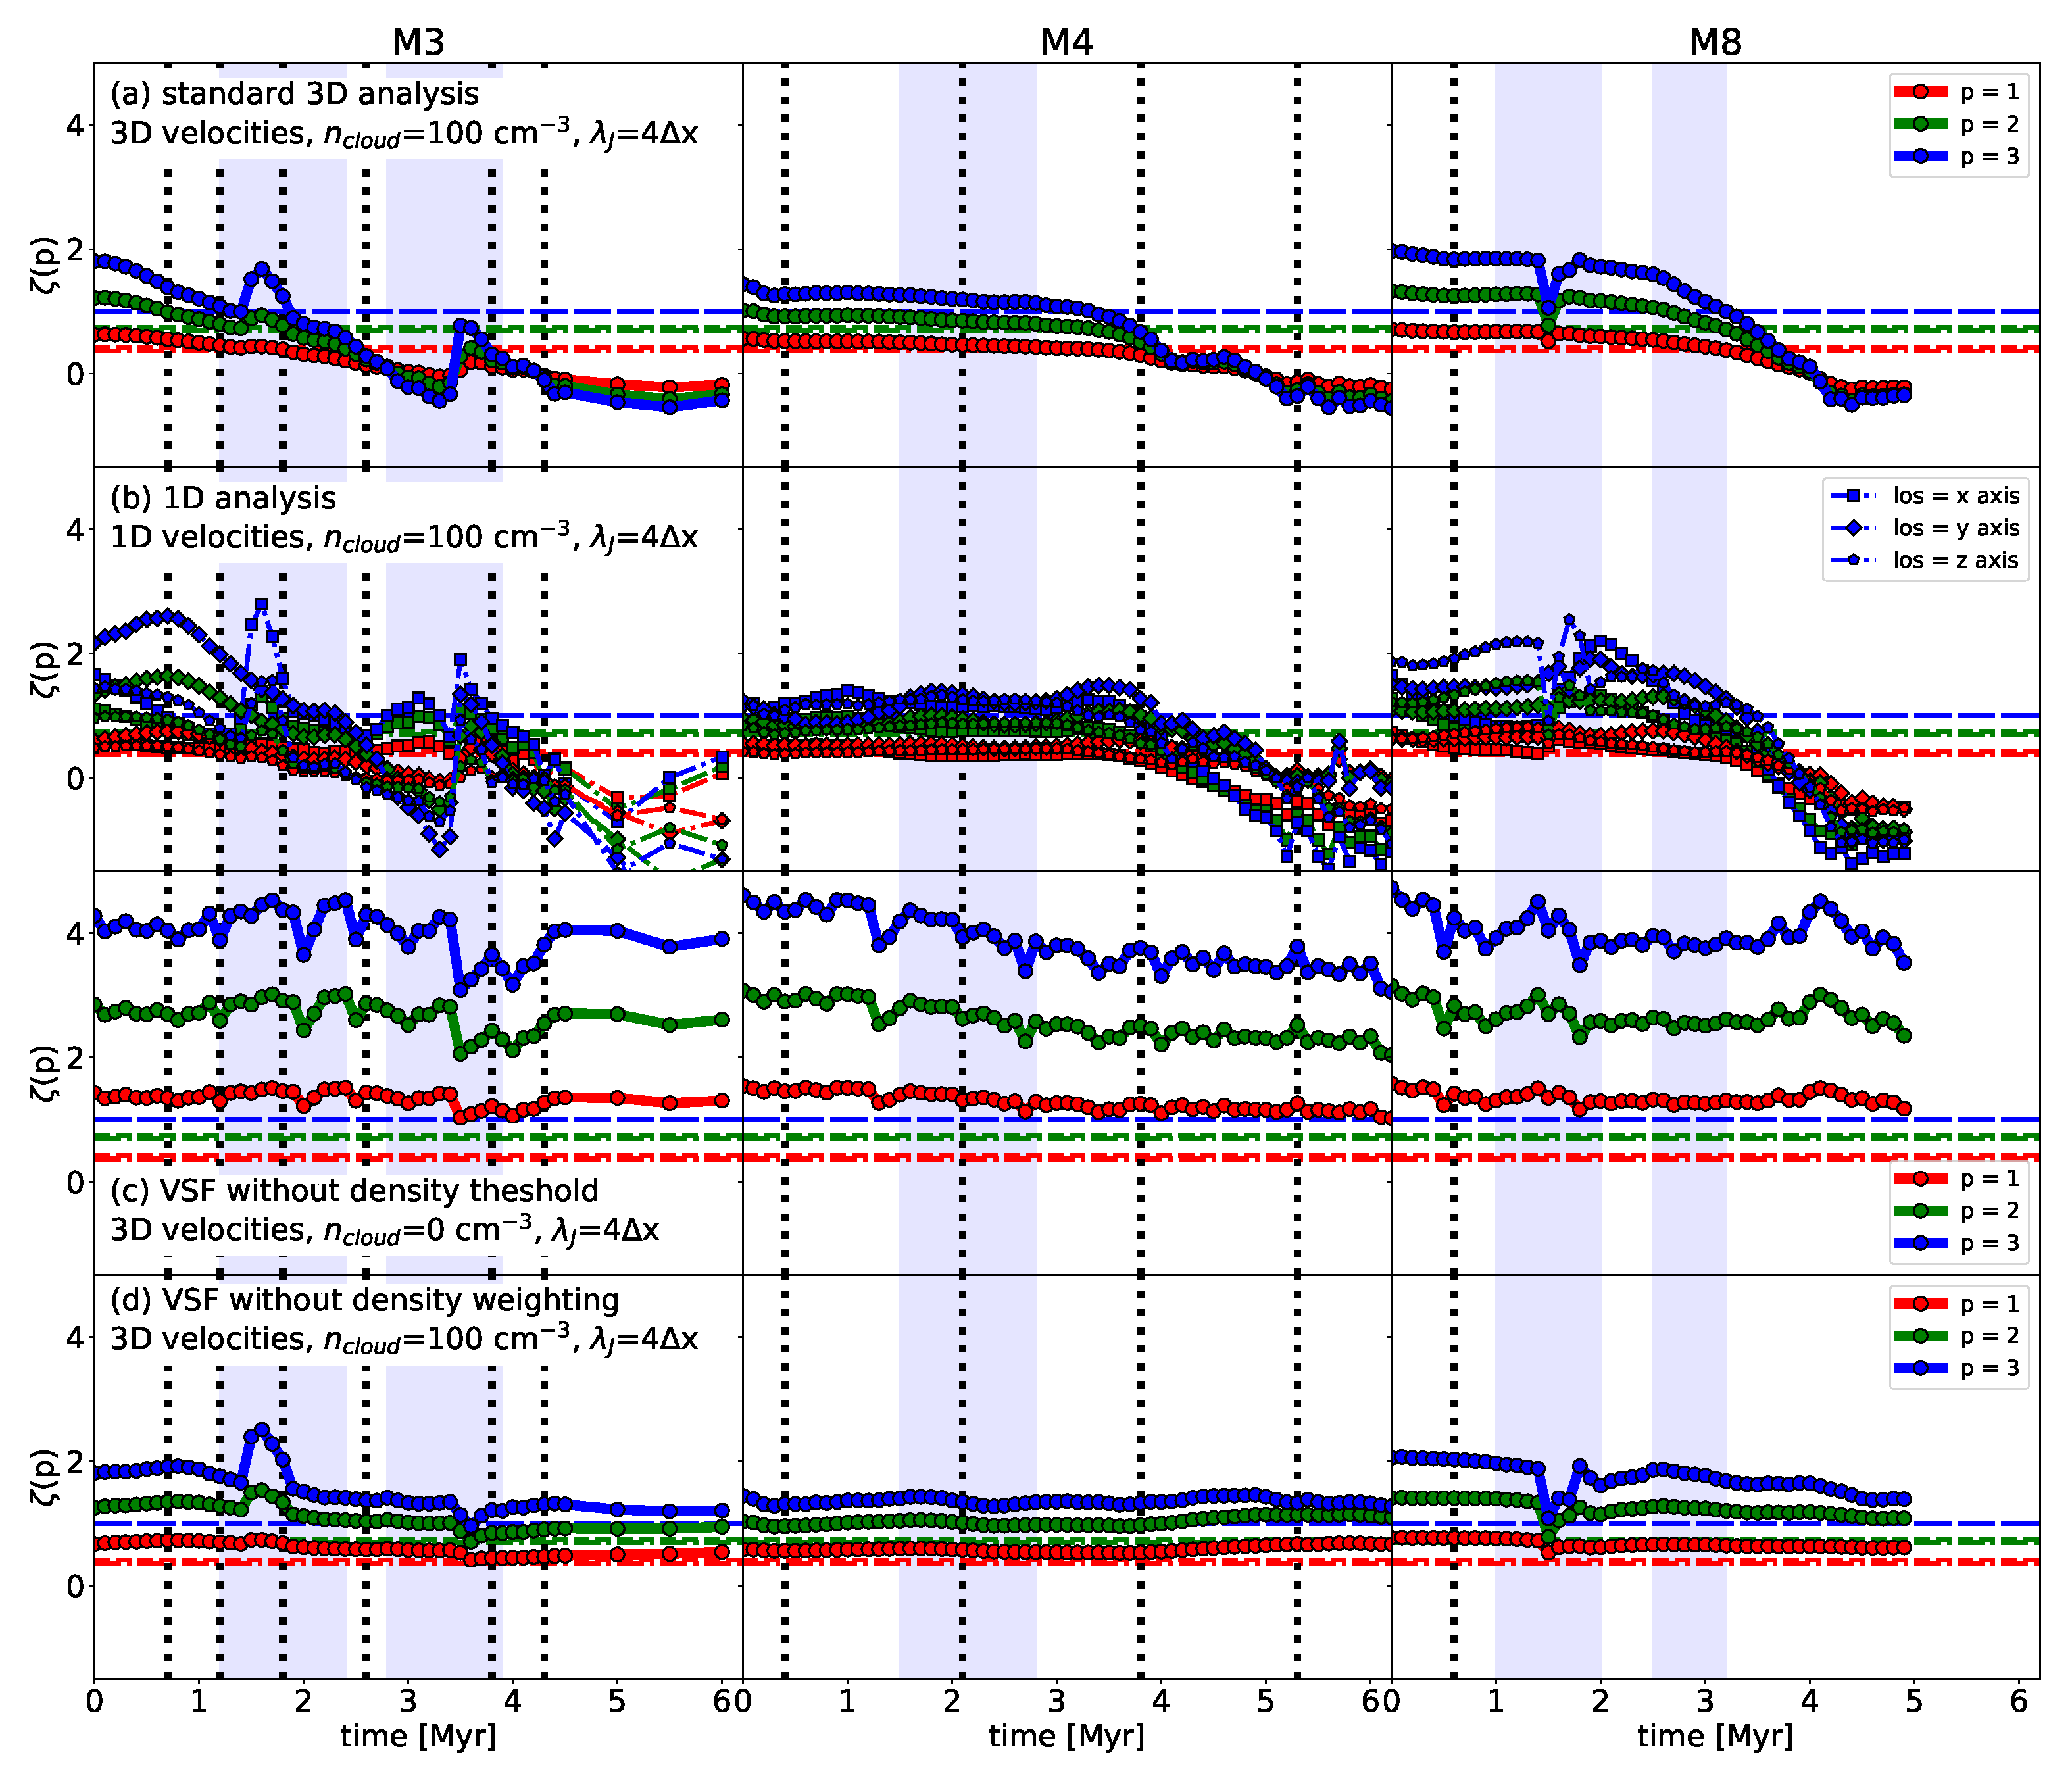
\includegraphics[width=\textwidth]{zeta_all_nojeans.pdf}
      \label{pic:results:zeta_all_nojeans}
  \end{subfigure}
  \begin{subfigure}[c]{\textwidth}
      \addtocounter{subfigure}{4}
      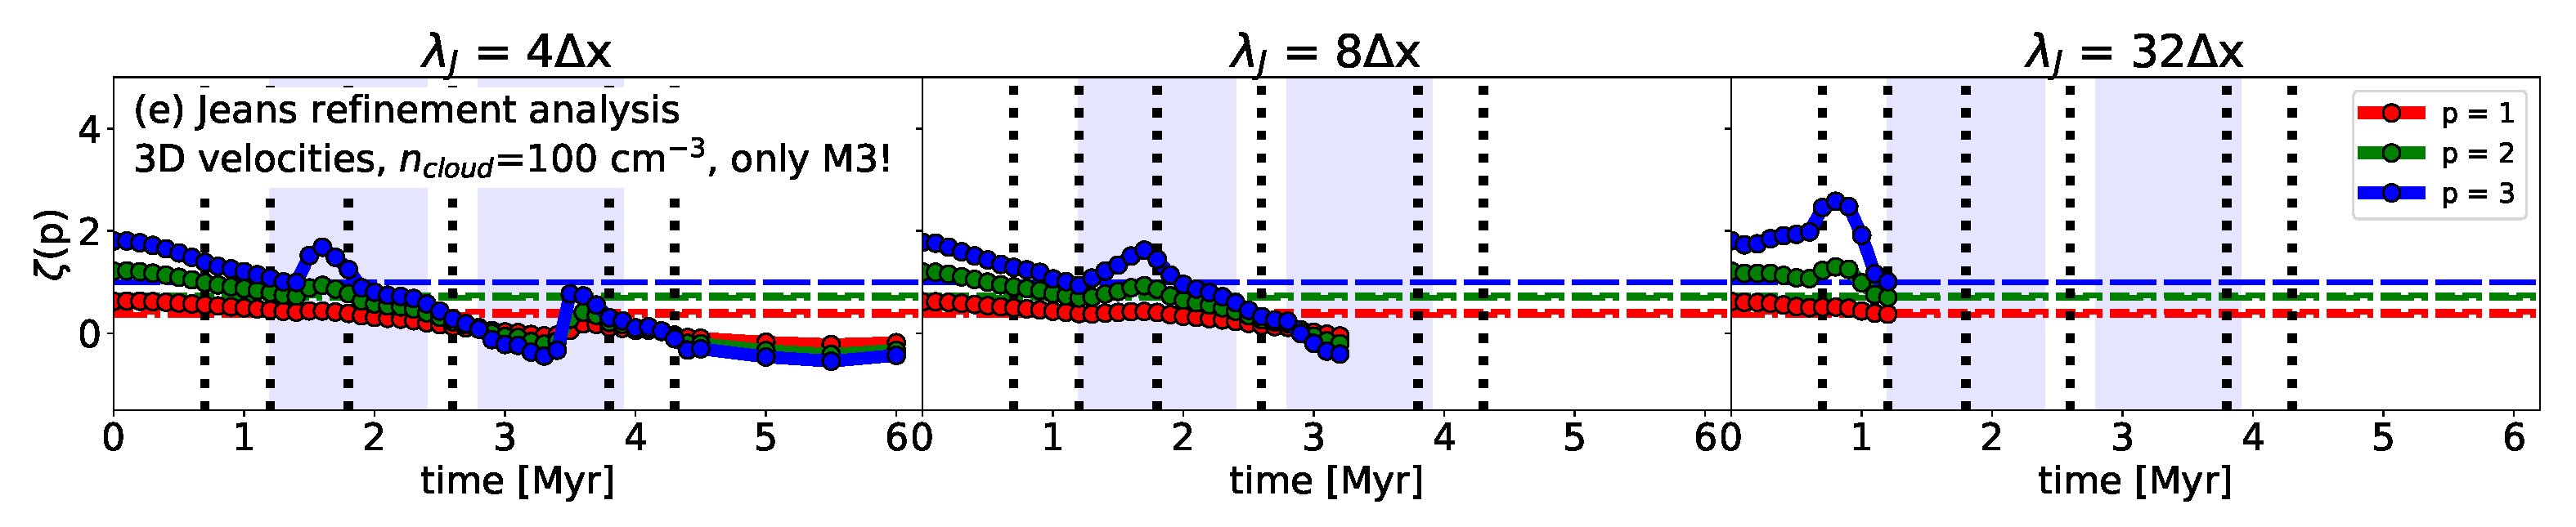
\includegraphics[width=\textwidth]{zeta_jeans.pdf}
      \label{pic:results:zeta_all_jeans}
  \end{subfigure}
  
  \caption{Time evolution of scaling exponent $\zeta(p)$ of the $p^\mathrm{th}$ order VSF. Panels (a)--(d) show the measurements for \texttt{M3}~(\textit{left}), \texttt{M4}~(\textit{middle}), and \texttt{M8}~(\textit{right}), respectively. Of these, (a) represents the standard analysis while the other rows illustrate the results of \textbf{different variations in the analysis as noted in the figures.} Panel (e) shows the values of $\zeta$ measured within \texttt{M3} as a function of the Jeans refinement level the cloud has been modelled with.  \textbf{Note that these more expensive runs were not run for as long as the fiducial run.  In all panels, the grey dotted vertical lines mark the times than a SN explodes in the vicinity of the corresponding cloud, while the blue areas indicate periods of enhanced mass accretion onto the clouds.} The coloured horizontal lines show the predicted values for \textbf{incompressible turbulence \citep[dash-dotted lines;][]{She1994} and for highly compressible, supersonic turbulence \citep[dashed lines;][]{Boldyrev2002}.}}
	\label{pic:results:zeta_all}
\end{figure*}

Fig.~\ref{pic:results:z_all}(a) shows the \textbf{corresponding} time evolution of the self-similarity parameter, $Z$. 
One sees that most of the time the measured values of $Z$ are in agreement or at least closely approaching the predicted values. 
\textbf{The occasional peaks in} $Z$ (for example, in \texttt{M4} at $t$~=~4.1~Myr) occur at times when the scaling exponents of the VSFs $\zeta(3)$ reach values close to or below 0.
The decreases in $Z$ (for example, in \texttt{M3} around $t$~=~1.8~Myr), on the other hand, occur when SN shocks hit and heavily impact the clouds, \textbf{producing stronger effects in higher order VSFs.}

\begin{figure*}[!htb]
	\centering  
  
  \begin{subfigure}[c]{\textwidth}
      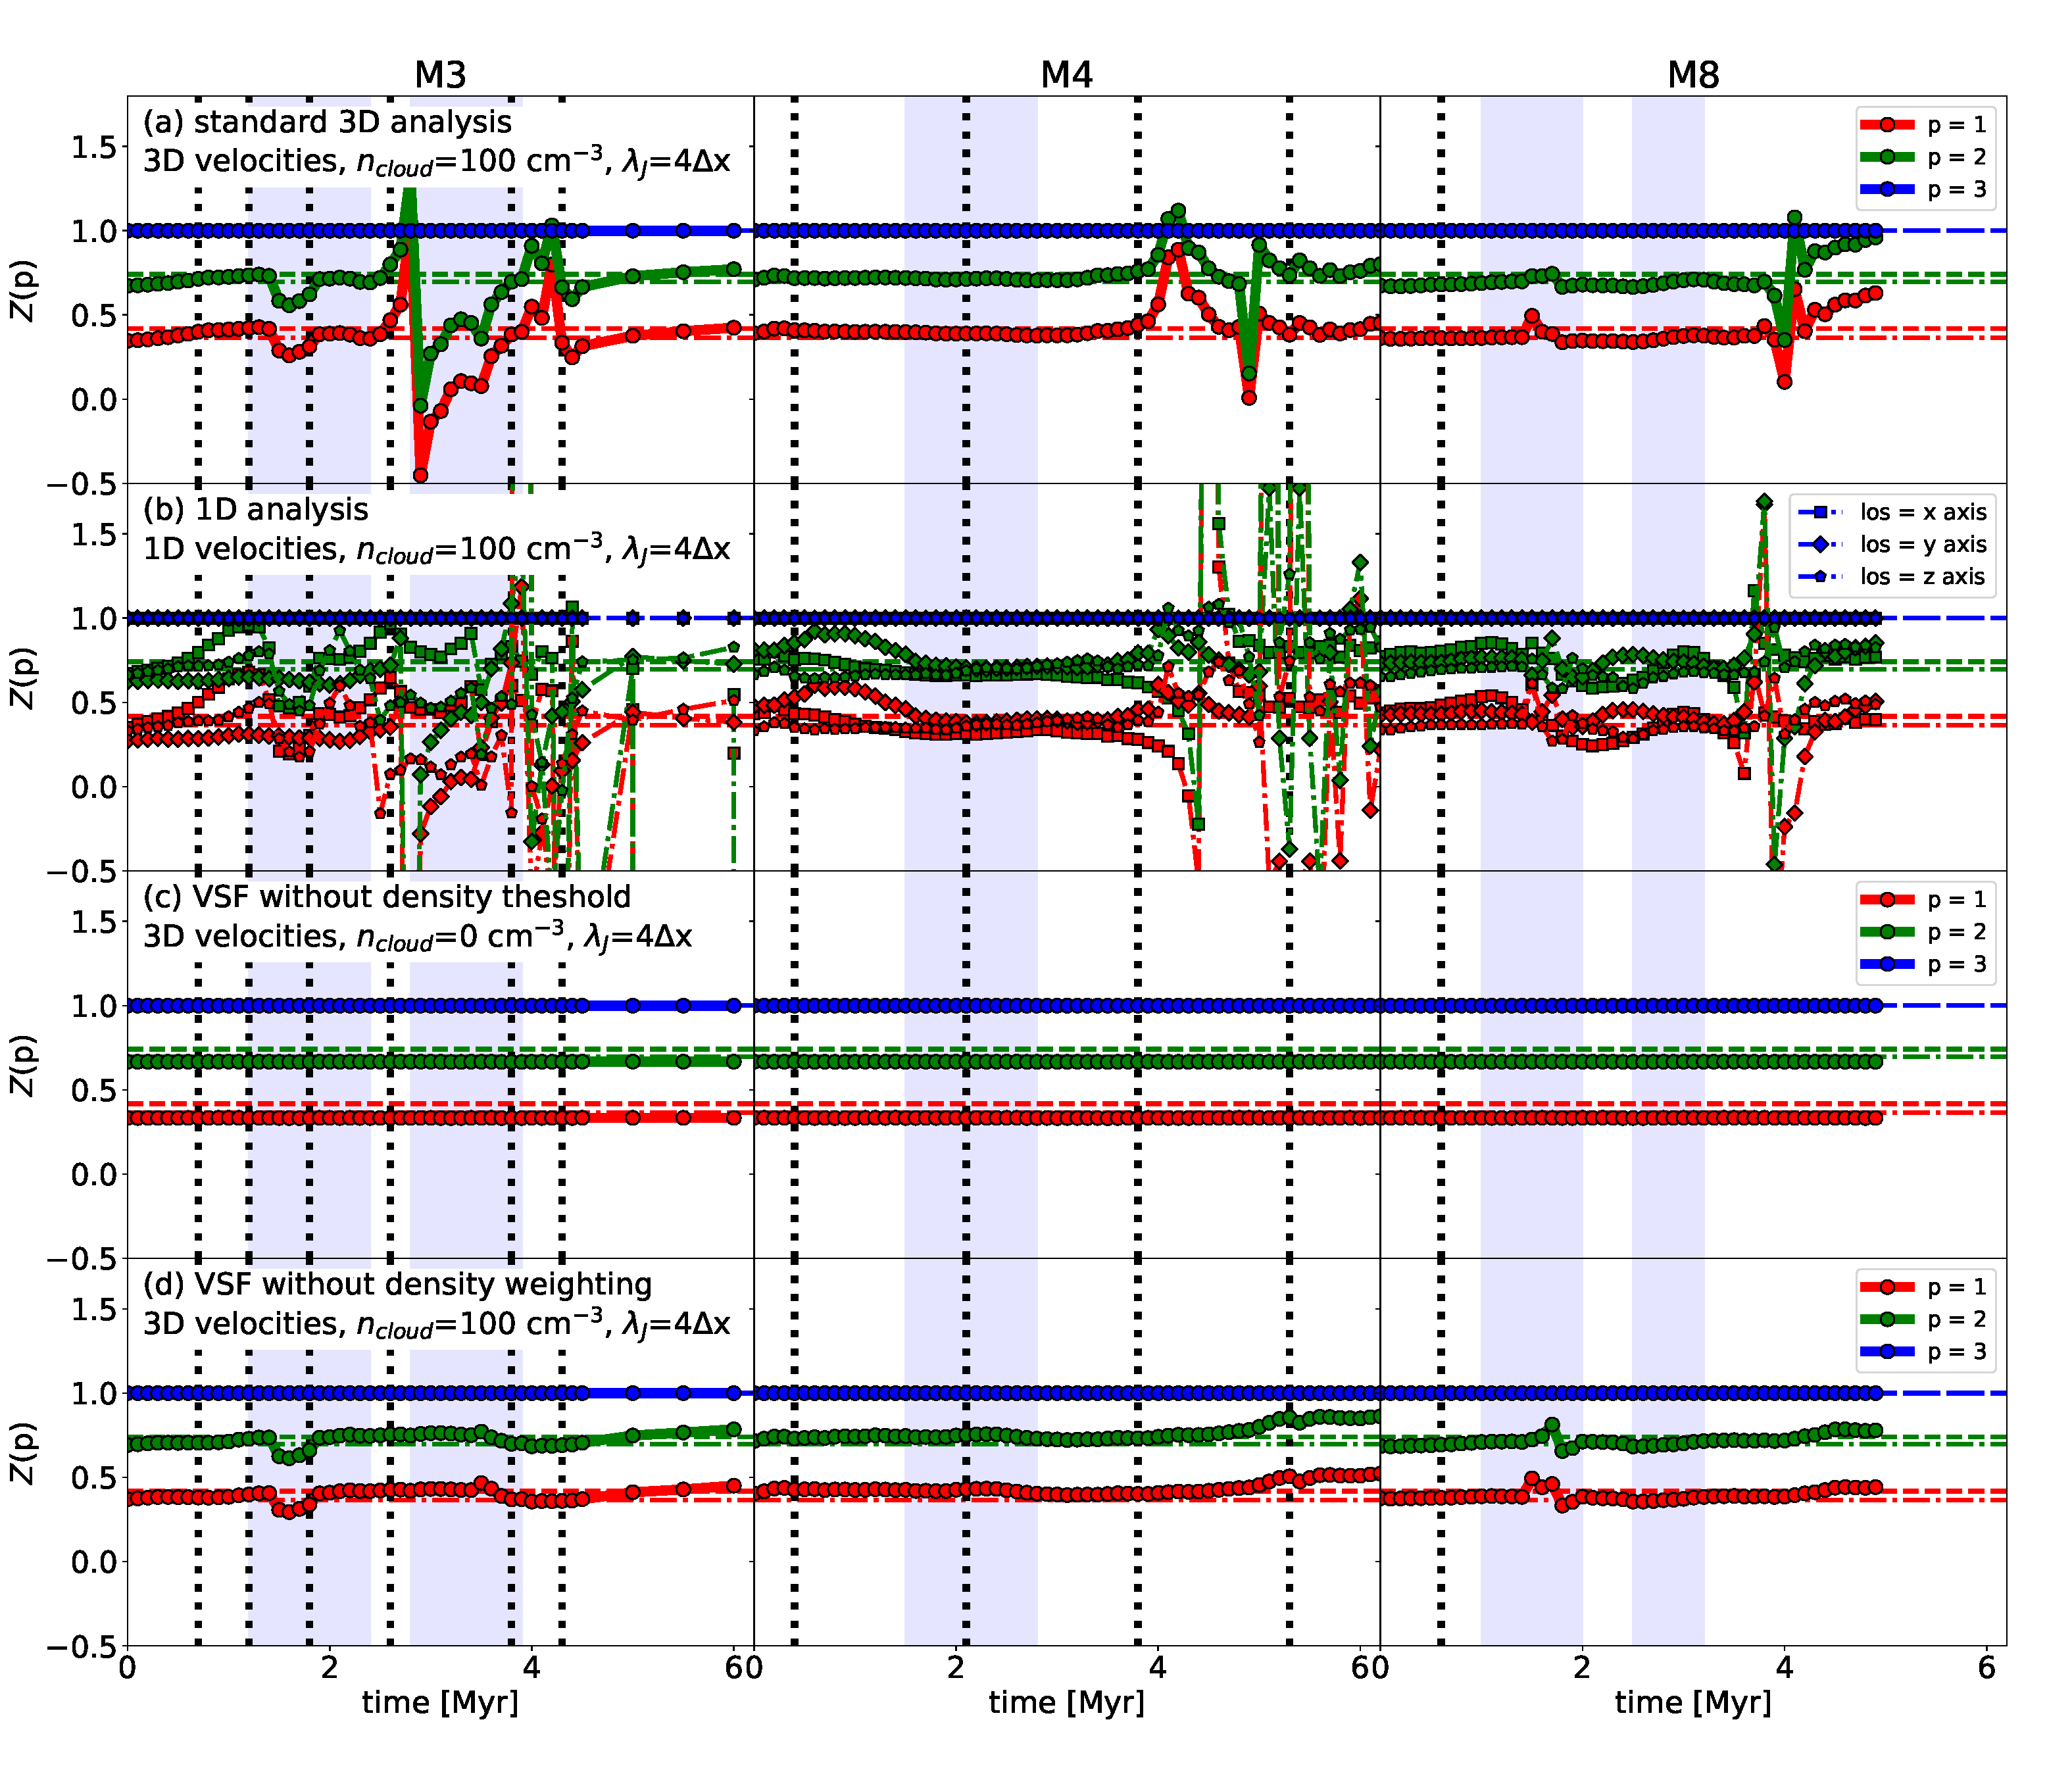
\includegraphics[width=\textwidth]{z_all_nojeans.pdf}
      \label{pic:results:z_all_nojeans}
  \end{subfigure}
  
  \begin{subfigure}[c]{\textwidth}
      \addtocounter{subfigure}{4}
      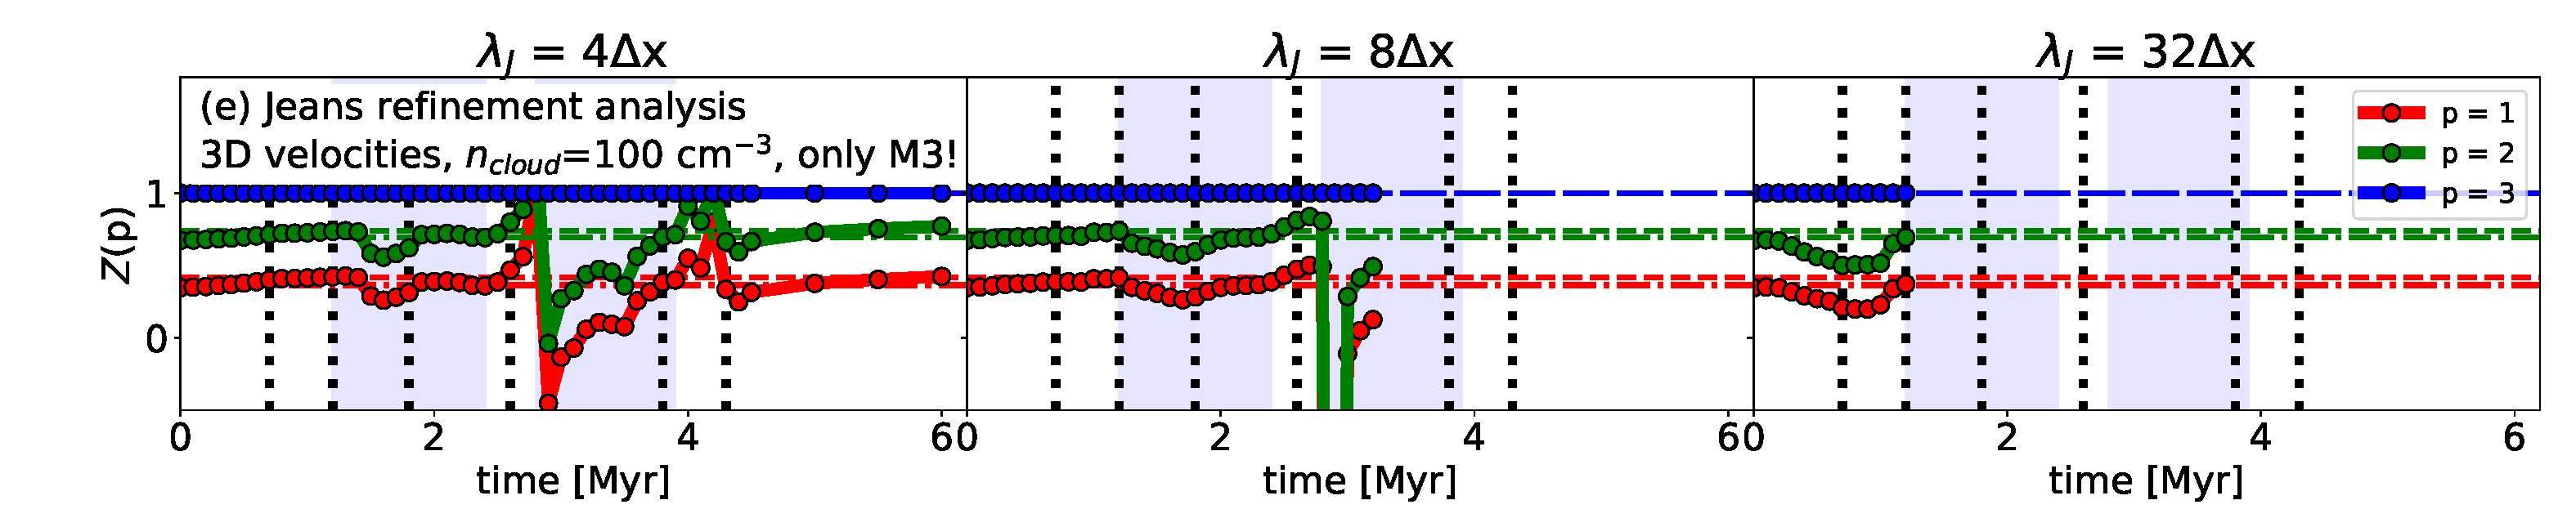
\includegraphics[width=\textwidth]{z_jeans.pdf}
      \label{pic:results:z_all_jeans}
  \end{subfigure}
  
  \caption{Like Fig.~\ref{pic:results:zeta_all}, but for the measured self-similarity parameter $Z = \zeta(p) / \zeta(3)$ of the $p^\mathrm{th}$ order VSF.}
	\label{pic:results:z_all}
\end{figure*}

In the rest of this section, we study how VSFs \textbf{computed in different ways compare to these density weighted results.}
We compare the findings with the results we have obtained with our original setup.
In Sect.~\ref{discussion}, we will discuss and interpret these results in more detail.


\subsection{Line-of-Sight VSF}\label{results:1d}

Previously, we have seen how the VSF behaves and evolves within the clouds.
By doing so, we derived the relative velocities based on the 3D velocity vectors \textbf{from the simulations.
However, observed VSFs can only be measured using line-of-sight velocities.}
Thus, in this subsection we investigate how VSFs derived from 1D relative velocities compare to the 3D VSFs presented before.

Figures~\ref{pic:results:zeta_all}(b) and~\ref{pic:results:z_all}(b) show measured $\zeta$ and $Z$, respectively, derived based on Eq.~(\ref{equ:results:def_vsf_1d}). 
We see that, in most of the cases, all 1D VSFs agree well with each other, as well as with the corresponding 3D VSFs.
Yet, there are cases in which the 1D VSF evolves temporarily or completely differently than the 3D VSF.
For example, the 1D VSF along the x-axis in \texttt{M3} initially behaves like the corresponding 3D VSF, though with lower absolute values of $\zeta$ (or higher values of $Z$).
However, during the period $t$~=~2.5--3.8~Myr the functions diverge. 
While the 3D $\zeta$ \textbf{decreases} further and switches sign, the $\zeta$ based on the 1D VSF along the $x$-axis shows a local maximum before converging with the 3D $\zeta$ again. 


\subsection{Density Thresholds}\label{results:densthres}

\textbf{We now examine the VSFs of the entire data cubes without setting a density threshold ($n_\mathrm{cloud}~=$~0~cm$^{-3}$).  Figure~\ref{pic:results:zeta_all}(c) shows $\zeta$, while Figure~\ref{pic:results:z_all}(c) shows $Z$ in this case.
These figures clearly illustrate that the measurements in the samples without density threshold completely differ from those with the density threshold.}
The measured values of $\zeta$ are much higher in the ISM than in the cloud-only sample.
Although we see a similar decline of $\zeta$ in \texttt{M4} and \texttt{M8} as the gas contracts under the influence of gravity in the vicinity of the clouds, $\zeta$ generally evolves differently here than \textbf{in the analysis that is focused on the clouds.}
We see a high rate of random fluctuations in the evolution of $\zeta$, as well.
Furthermore, contrary to all of our other test scenarios, we see here that all $Z$ are constant in time and within all clouds, with values slightly lower than those predicted by \citet{She1994} for \textbf{incompressible} flows.  
\textbf{This is consistent with the high sound speed in the hot gas that fills most of the volume of the computational box, which results in subsonic flows predominating.}


\subsection{Density Weighting}\label{results:densweight}

As mentioned in Sect.~\ref{methods:vsf}, Eq.~(\ref{equ:method:def_vsf}) represents the definition of the density-weighted VSF.
\textbf{While this represents the observational situation better, the theoretical predictions were developed for the unweighted statistic.  Thus a comparison of results for the two variations in our model is of interest. }
There are a few studies that have targeted this question 
\citep[e.g.,][]{Benzi1993,Schmidt2008, Benzi2010,Gotoh2002}.  
However, all of them considered \textbf{isotropic, homeogeneous, turbulent flows} that are not comparable to our clouds.
\citet{Padoan2016a} use both methods, but not on the same set of data. 

In this section, we investigate the influence of density weighting on VSFs by repeating the original analysis with the non-weighted VSF given by Eq.~\ref{equ:method:def_vsf}.
Figs.~\ref{pic:results:zeta_all}(d) and~\ref{pic:results:z_all}(d) show the measured values of $\zeta$ and $Z$ derived from the non-weighted VSFs, respectively.

Comparing the weighted and non-weighted samples, we see the following:
The non-weighted $\zeta$ (Fig.~\ref{pic:results:zeta_all}d) traces the interactions between the gas of the clouds and the SN shocks in the same way as occurs for the density-weighted VSF.
In \texttt{M3} and \texttt{M8} we also see that the values of $\zeta$ decrease as the clouds evolve, yet not as fast as they do in the density-weighted VSFs. 
The measurements in \texttt{M4}, however, are almost constant over time. 
In all the cases, the values of $\zeta$ never \textbf{decrease} below 0.5; a behaviour that clearly differs from what we have observed in the density-weighted VSFs. 
\textbf{The density weighting weakens the influence of the highly compressible flows in the densest regions, but not so much as in the case with no density threshold. 
Consequently, the evolution of $Z$s (see Fig.~\ref{pic:results:z_all}d) becomes smoother, as well, as there is no sign inversion of $\zeta$.
As a result the values of $Z$ fluctuate slightly when shocks hit, and otherwise vary between the compressible and incompressible limits.}



\subsection{Jeans Length Refinement}\label{results:refinement}

\textbf{The results we have discussed so far are based on simulation data presented in \citetalias{IbanezMejia2016} and \citetalias{IbanezMejia2017}.
Due to the huge computational expense of the variety of physical and numerical processes (fluid dynamics, AMR, supernovae, magnetic fields, radiative heating and cooling, and many more) within those simulations, though, they have required some compromises.
One of these compromises was the Jeans refinement criterion used as part of the AMR mechanisms.
The authors resolved local Jeans lengths by only four cells ($\lambda_J=4\Delta{}x$).
This is the minimal requirement for modelling self-gravitating gas in disks in order to avoid artificial fragmentation \citep{Truelove1998}. 
Other studies, for example by \citet{Turk2012}, have shown that a significantly higher refinement is needed to reliably resolve turbulent structures and flows within disks to resolve turbulence.  In our case, the key question is how quickly the turbulent cascade fills in after the multiple steps of refinement to higher resolution required to develop the high resolution cubes we use.  
Although we have a different physical situtation, the earlier results still emphasize the importance of how well the Jeans length is resolved.}

In the appendix of \citetalias{IbanezMejia2017}, the authors examine the effect the number of cells used for the Jeans refinement has on the measured kinetic energy.
For this, they have rerun the simulations of \texttt{M3} twice; 
once with $\lambda_J=8\Delta{}x$ for the first 3~Myr after self-gravity was activated, and once with $\lambda_J=32\Delta{}x$ for the first megayear of the cloud's evolution.
The authors show that the $\lambda_J=32\Delta{}x$ simulations smoothly \textbf{recover} the energy power spectrum on all scales already after this first megayear.
The other two setups do this, as well, \textbf{but only over longer timescales.}
This is why one can only reliably trust the findings in this paper after the clouds have evolved for approximately 1.5~Myr \citep[see also][]{IbanezMejia2017,Seifried2017b}.

Furthermore, \citetalias{IbanezMejia2017} calculated the difference in the cloud's total kinetic energy as a function of time and refinement level.
They found that the $\lambda_J = 4\Delta{}x$ simulations miss a significant amount of kinetic energy, namely up to 13\% compared to $\lambda_J = 8\Delta{}x$ and 33\% compared to $\lambda_J = 32\Delta{}x$.
However, they also observed that these differences peak around $t=0.5$~Myr and decrease afterwards, as the $\lambda_J = 4\Delta{}x$ and $\lambda_J = 8\Delta{}x$ simulations adjust to the new refinement levels.
Thus, the results we have derived from the $\lambda_J = 4\Delta{}x$ simulations need to be evaluated with respect to this lack of turbulent energy, although the clouds' dynamics remains dominated by gravitational collapse.
It also means that the $\lambda_J = 4\Delta{}x$ data become more reliable the longer the simulations evolve.

In order to study  how the level of Jeans refinement influences the behaviour of the VSFs, we investigate the \texttt{M3} data of the $\lambda_J = 8\Delta{}x$ and $\lambda_J = 32\Delta{}x$ simulations.
Figs.~\ref{pic:results:zeta_all}e and \ref{pic:results:z_all}e show $\zeta$ and $Z$ for  $\lambda_J = 8\Delta{}x$ and $\lambda_J = 32\Delta{}x$.
In Fig.~\ref{pic:results:jeans_comp} we directly compare the measurements of all refinement levels relative to $\lambda_J = 4\Delta{}x$.

$\lambda_J = 8\Delta{}x$ shows the same behaviour as $\lambda_J = 4\Delta{}x$, with values in both samples being in good agreement as the top panel of Fig.~\ref{pic:results:jeans_comp} demonstrates. 
Over the entire observed time span, the measured values of $\zeta$ decrease as the VSF become flatter.
At the time the SNe interact with the cloud, \textbf{over the course of about a megayear after traveling across the distance from the point of explosion to the cloud, the VSFs steeply increase toward larger scales causing values of $\zeta$ (Fig.~\ref{pic:results:zeta_all}e) to jump.}
Compared to the $\lambda_J = 4\Delta{}x$ sample, the peak in $\zeta$ is smoother and lasts longer \textbf{at higher Jeans resolution}.

\textbf{These same effects can be seen in Fig.~\ref{pic:results:z_all}e where the drop of $Z$ due to the SN shock lasts longer than it did for} $\lambda_J = 4\Delta{}x$. 
Besides this, the time evolution of $Z$ for $\lambda_J = 8\Delta{}x$ is as sensitive to the turbulence-related events as it was for $\lambda_J = 4\Delta{}x$.
The divergence produced when gravity has transferred the majority of power to smaller scales occurs at the same time. 
\textbf{The actual} depth of the drop is a numerical artefact caused by $\zeta(3)$ being equal or close to zero at this very time step. 

The picture changes when we analyse the VSFs based on the $\lambda_J = 32\Delta{}x$ runs (Figs.~\ref{pic:results:zeta_all}e,~\ref{pic:results:z_all}e, and~\ref{pic:results:jeans_comp}).
Here one sees that the measured values of both $\zeta$ (Fig.~\ref{pic:results:zeta_all}e) and $Z$ (Fig.~\ref{pic:results:z_all}e) are similar to those for $\lambda_J = 4\Delta{}x$ for the first 0.2~Myr.
After this short period, though, the evolution of $\zeta$ diverge. 
While $\zeta(1)$ and $\zeta(2)$ continue to decrease \textbf{similar to $\lambda_J = 4\Delta{}x$ but at lower rate,} $\zeta(3)$ increases until it peaks at $t=0.8$~Myr and falls steeply again.
This divergence has notable impact on the evolution of $Z$, as well. 
The bottom panel of Fig.~\ref{pic:results:jeans_comp} illustrates the different evolutions of measured $\zeta$ and $Z$ in the two simulations more clearly.
One sees that the differences between the samples follow the same pattern for all orders of $p$.
The differences, though, increase with the order:
While the values for $\zeta(1)$ are still in good agreement, the measured values of $\zeta(2)$ and $\zeta(3)$ for $\lambda_J = 32\Delta{}x$ are 40\% and 100\% higher than those measured for $\lambda_J = 4\Delta{}x$, respectively.
Consequently, this causes differences in $Z(p)$ of 30--52\% between the simulations.
At $t$~=~1.2~Myr, the last time step of this sample, the values of all $\zeta$ equal the measurements of $\lambda_J = 4\Delta{}x$ again.
\textbf{As the cost of extending the $\lambda_J = 32\Delta{}x$ simulation is prohibitive, we cannot determine whether this agreement will continue.}

\begin{figure*}
	\centering
    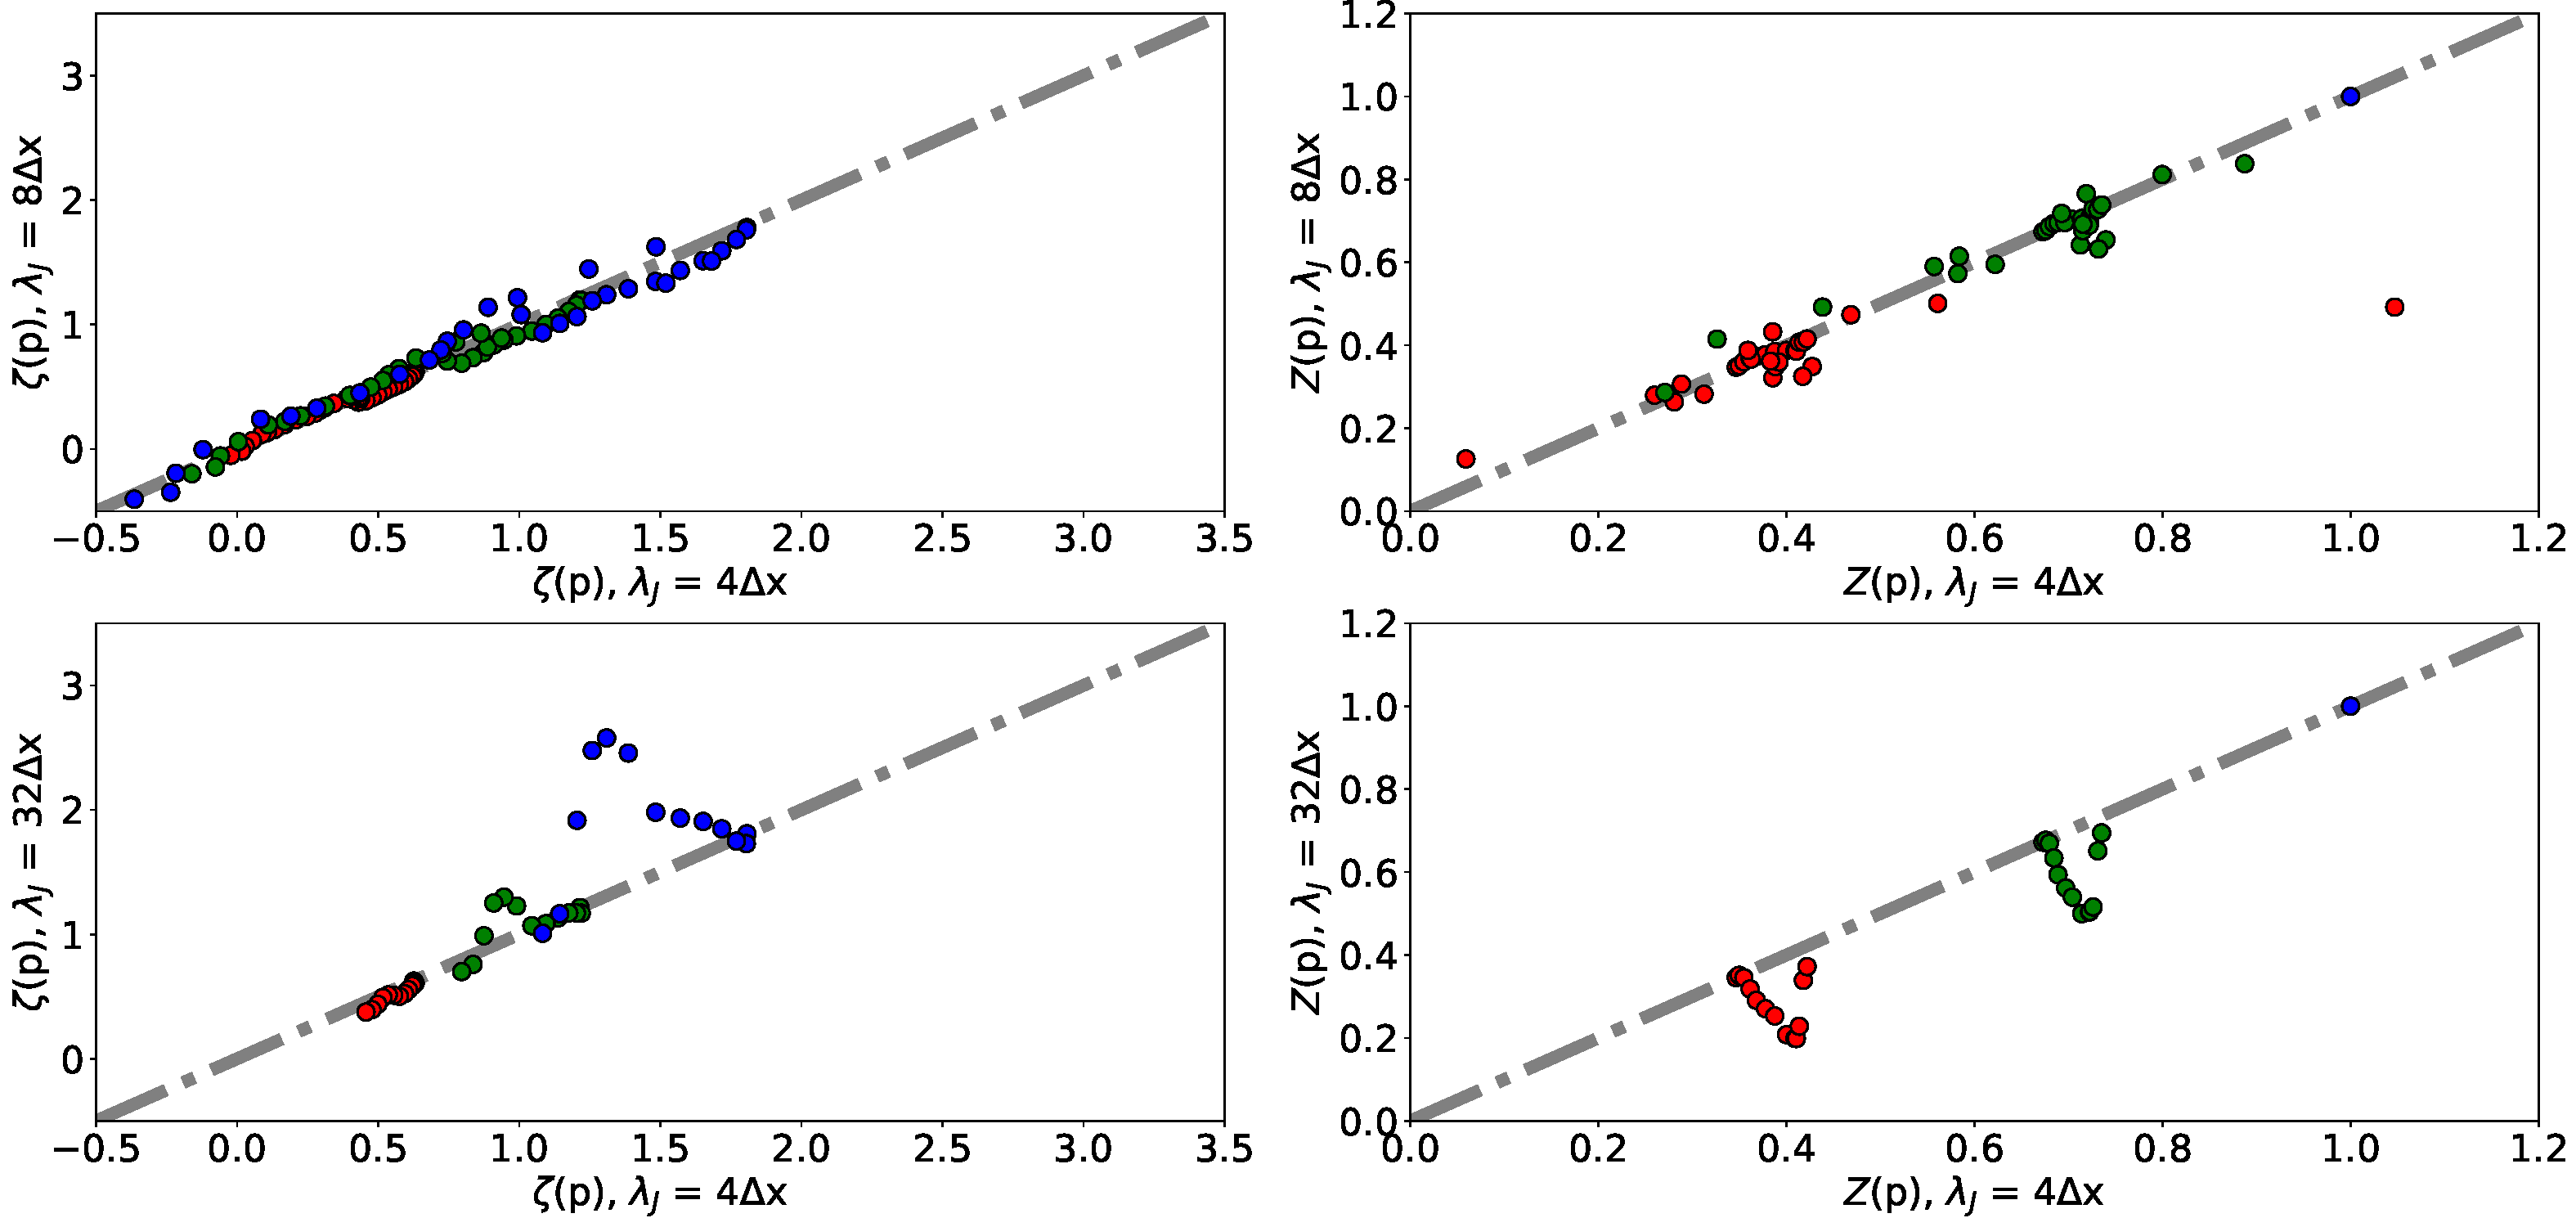
\includegraphics[width=\textwidth]{comp_jeans.pdf}
    \caption{Comparison of VSF scaling exponents, $\zeta$ (\textit{left}), and self-similarity parameters, $Z$ (\textit{right}), depending on the Jeans refinement of the simulation runs the data are based on. The abscissas give values from $\lambda_J = 4\Delta{}x$, while the ordinates give values from $\lambda_J = 8\Delta{}x$ (\textit{top}) and $\lambda_J = 32\Delta{}x$ (\textit{bottom}). All data points refer to the \texttt{M3} cloud and represent \textbf{different lags in} the same time step in the respective simulations. 
    }
    \label{pic:results:jeans_comp}
\end{figure*}

